\documentclass{article}

% Required packages (merged from hw5_template.tex and hw6_questions.tex)
\usepackage{amssymb}
\usepackage{amsmath}
\usepackage{graphicx}
\usepackage{geometry}
\usepackage{tikz}
\usepackage{array}
\usepackage{booktabs}
\usepackage{enumitem}
\usepackage{listings}
\usepackage{xcolor}
\usepackage{fancyhdr}
\usepackage{float}
\usepackage{subcaption}
\usepackage{comment}
\usepackage{algorithm}
\usepackage{algpseudocode}
\usepackage{caption}
\usepackage{siunitx}
\usepackage{hyperref}
\usetikzlibrary{arrows.meta, positioning} % Required for hw6 diagrams

% Set page geometry
\geometry{a4paper, margin=1in}

% Configure listings for Python
\lstset{
  language=Python,
  basicstyle=\ttfamily\footnotesize,
  numbers=left,
  numberstyle=\tiny\color{gray},
  frame=single,
  breaklines=true,
  breakatwhitespace=true,
  captionpos=b,
  tabsize=4,
  showspaces=false,
  showstringspaces=false,
  showtabs=false,
  commentstyle=\color{gray}\textit,
  keywordstyle=\color{blue}\bfseries,
  stringstyle=\color{red}
}

\begin{document}

\pagestyle{fancy}
\chead{DSC 257: Unsupervised Learning (Fall 2025)}
\lhead{Homework 7}
\rhead{Randall Rogers}

%------------------
% Solution for 1(a)
%------------------
\subsection*{Solution 1}
\noindent\rule{\textwidth}{0.4pt}\\

\subsubsection*{Solution 1 (a)}
\begin{flushleft}
    Given the probability distribution $P$ over binary variables $x_1, \ldots, x_6 \in \{0, 1\}$ has the following form:
\end{flushleft}
$$
P(x_1, \ldots, x_6) = \frac{1}{Z} \psi(x_1, x_2)\psi(x_2, x_3)\psi(x_3, x_4)\psi(x_4, x_5)\psi(x_5, x_6)\psi(x_6, x_1)
$$
\begin{flushleft}
    where for $a, b \in \{0, 1\}$,
\end{flushleft}
$$
\psi(a, b) = \begin{cases}
1 & \text{if } a = b\\
0.5 & \text{otherwise}
\end{cases}
$$
\begin{flushleft}
    From the Hammersley-Clifford theorem the potential terms are:
\end{flushleft}
$$\psi(x_1, x_2) \implies \text{ edge between } x_1 \text{ and } x_2 \qquad \psi(x_4, x_5) \implies \text{ edge between } x_4 \text{ and } x_5$$
$$\psi(x_2, x_3) \implies \text{ edge between } x_2 \text{ and } x_3 \qquad \psi(x_5, x_6) \implies \text{ edge between } x_5 \text{ and } x_6$$
$$\psi(x_3, x_4) \implies \text{ edge between } x_3 \text{ and } x_4 \qquad \psi(x_6, x_1) \implies \text{ edge between } x_6 \text{ and } x_1$$
\begin{flushleft}
    Now, with the information above, we can draw the minimal undirected graph.
\end{flushleft}

\begin{center}
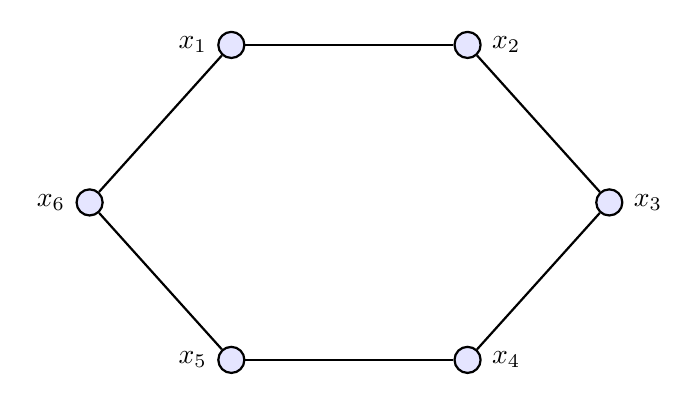
\begin{tikzpicture}[node distance=2cm, thick]
    % Nodes
    \node[circle, draw, fill=blue!10, label=left:$x_1$] (x1) at (0, 2) {};
    \node[circle, draw, fill=blue!10, label=right:$x_2$] (x2) at (3, 2) {};
    \node[circle, draw, fill=blue!10, label=right:$x_3$] (x3) at (4.8, 0) {};
    \node[circle, draw, fill=blue!10, label=right:$x_4$] (x4) at (3, -2) {};
    \node[circle, draw, fill=blue!10, label=left:$x_5$] (x5) at (0, -2) {};
    \node[circle, draw, fill=blue!10, label=left:$x_6$] (x6) at (-1.8, 0) {};

    % Edges
    \draw (x1) -- (x2);
    \draw (x2) -- (x3);
    \draw (x3) -- (x4);
    \draw (x4) -- (x5);
    \draw (x5) -- (x6);
    \draw (x6) -- (x1);
\end{tikzpicture}
\end{center}

\subsubsection*{\normalfont}{$\therefore$ The minimal undirected graph given the probability distribution $P$ is seen above.}

\noindent\rule{\textwidth}{0.4pt}\\

\newpage

%------------------
% Solution for 1(b)
%------------------
\subsection*{Solution 1}
\noindent\rule{\textwidth}{0.4pt}\\
\subsubsection*{Solution 1 (b)}
\begin{flushleft}
    Given the probability distribution $P$ over binary variables $x_1, \ldots, x_6 \in \{0, 1\}$ has the following form:
\end{flushleft}
$$
P(x_1, \ldots, x_6) = \frac{1}{Z} \psi(x_1, x_2)\psi(x_2, x_3)\psi(x_3, x_4)\psi(x_4, x_5)\psi(x_5, x_6)\psi(x_6, x_1)
$$
\begin{flushleft}
    where for $a, b \in \{0, 1\}$, and
\end{flushleft}
$$
\psi(a, b) = \begin{cases}
1 & \text{if } a = b\\
0.5 & \text{otherwise}
\end{cases}
$$
\begin{flushleft}
    To find the $x$ that maximizes $P(X)$ we have the following:
\end{flushleft}
\begin{align*}
    \arg\max_{x} P(x) &= \arg\max_{x} \left[ \frac{1}{Z} \prod_{i=1}^{5} \psi(x_i, x_{i+1}) \cdot \psi(x_6, x_1) \right]
\end{align*}
\begin{flushleft}
    Since the partition function $Z$ is a positive constant,we can ignore it and maximizing $P(x)$ becomes:
\end{flushleft}
\begin{align*}
    \arg\max_{x} P(x) &= \arg\max_{x} \left[ \psi(x_1, x_2)\psi(x_2, x_3)\psi(x_3, x_4)\psi(x_4, x_5)\psi(x_5, x_6)\psi(x_6, x_1) \right]
\end{align*}
\begin{flushleft}
    Given $\psi(a,b)$ is maximized at, the maximum possible value for any single potential is $\psi(a, a) = 1$.
\end{flushleft}

$$\psi(a, b) = 1 \text{ where } a=b$$
Now, maximizing the value of each term in the product yeilds:
$$\psi(x_1, x_2) = 1 \implies  x_1 = x_2 \qquad \psi(x_4, x_5) = 1 \implies  x_4 = x_5$$
$$\psi(x_2, x_3) = 1 \implies  x_2 = x_3 \qquad \psi(x_5, x_6) = 1 \implies  x_5 = x_6$$
$$\psi(x_3, x_4) = 1 \implies  x_3 = x_4 \qquad \psi(x_6, x_1) = 1 \implies  x_6 = x_1$$

\begin{flushleft}
    Hence, $x_1 = x_2 = x_3 = x_4 = x_5 = x_6$ is the condition for the configuration that maximizes of $P(x)$. 
\end{flushleft}

\subsubsection*{\normalfont}{$\therefore$ Since $x_i$ can only be $0$ or $1$ ($x_i \in \{0,1\}$), the configurations that maximize $P(x)$ are:}
$$x = (0, 0, 0, 0, 0, 0) \qquad \text{and} \qquad x = (1, 1, 1, 1, 1, 1)$$

\noindent\rule{\textwidth}{0.4pt}\\

\newpage

%------------------
% Solution for 1(c)
%------------------
\subsection*{Solution 1}
\noindent\rule{\textwidth}{0.4pt}\\
\subsubsection*{Solution 1 (c)}
\begin{flushleft}
    Given the probability distribution $P$ over binary variables $x_1, \ldots, x_6 \in \{0, 1\}$ has the following form:
\end{flushleft}
$$
P(x_1, \ldots, x_6) = \frac{1}{Z} \psi(x_1, x_2)\psi(x_2, x_3)\psi(x_3, x_4)\psi(x_4, x_5)\psi(x_5, x_6)\psi(x_6, x_1)
$$
\begin{flushleft}
    where for $a, b \in \{0, 1\}$, and
\end{flushleft}
$$
\psi(a, b) = \begin{cases}
1 & \text{if } a = b\\
0.5 & \text{otherwise}
\end{cases}
$$
\begin{flushleft}
    To find the $x$ that minimizes $P(X)$ we have the following:
\end{flushleft}
\begin{align*}
    \arg\min_{x} P(x) &= \arg\min_{x} \left[ \frac{1}{Z} \prod_{i=1}^{5} \psi(x_i, x_{i+1}) \cdot \psi(x_6, x_1) \right]
\end{align*}
\begin{flushleft}
    Since the partition function $Z$ is a positive constant,we can ignore it and minimumizing $P(x)$ becomes:
\end{flushleft}
\begin{align*}
    \arg\min_{x} P(x) &= \arg\min_{x} \left[ \psi(x_1, x_2)\psi(x_2, x_3)\psi(x_3, x_4)\psi(x_4, x_5)\psi(x_5, x_6)\psi(x_6, x_1) \right]
\end{align*}
\begin{flushleft}
    Given $\psi(a,b)$ is minimized at:
\end{flushleft}
$$\psi(a, b) = 0.5 \text{ where } a \neq b$$
Now, minimizing the value of each term in the product yeilds:
$$\psi(x_1, x_2) = 0.5 \implies  x_1 \neq x_2 \implies x_1 = 0 , x_2 = 1 \text{ OR } x_1 = 1 , x_2 = 0 $$
$$\psi(x_2, x_3) = 0.5 \implies  x_2 \neq x_3 \implies x_2 = 0 , x_3 = 1 \text{ OR } x_2 = 1 , x_3 = 0 $$
$$\psi(x_3, x_4) = 0.5 \implies  x_3 \neq x_4 \implies x_3 = 0 , x_4 = 1 \text{ OR } x_3 = 1 , x_4 = 0 $$
$$\psi(x_4, x_5) = 0.5 \implies  x_4 \neq x_5 \implies x_4 = 0 , x_5 = 1 \text{ OR } x_4 = 1 , x_5 = 0 $$
$$\psi(x_5, x_6) = 0.5 \implies  x_5 \neq x_6 \implies x_5 = 0 , x_6 = 1 \text{ OR } x_5 = 1 , x_6 = 0 $$
$$\psi(x_6, x_1) = 0.5 \implies  x_6 \neq x_1 \implies x_6 = 0 , x_1 = 1 \text{ OR } x_6 = 1 , x_1 = 0 $$
\begin{flushleft}
    Hence, the conditions for the configuration that minimumizes of $P(x)$ are: 
\end{flushleft}
$$x = (0, 1, 0, 1, 0, 1) \qquad \text{ and } \qquad x = (1, 0, 1, 0, 1, 0)$$

\subsubsection*{\normalfont}{$\therefore$ Since $x_i$ can only be $0$ or $1$ ($x_i \in \{0,1\}$), and $a \neq b$ the configurations that maximize $P(x)$ are:}
$$x = (0, 1, 0, 1, 0, 1) \qquad \text{ and } \qquad x = (1, 0, 1, 0, 1, 0)$$

\noindent\rule{\textwidth}{0.4pt}\\

\newpage

%------------------
% Solution for 2(a)
%------------------
\subsection*{Solution 2}
\noindent\rule{\textwidth}{0.4pt}\\

\subsubsection*{Solution 2 (a)}
We will test for independence by finding a counterexample. Let's use $a=0$ and $c=1$.
\begin{itemize}
    \item $A=0$ is the event "Tom does not win his first game."
    \item $C=1$ is the event "Tom wins all three of his games."
\end{itemize}
The event $C=1$ (winning all three) requires winning Game 1. The event $A=0$ requires losing Game 1. These two events are mutually exclusive, so they cannot happen at the same time.

Therefore, the joint probability is $\Pr(A=0, C=1) = 0$.

Now, we check the product of the marginal probabilities, $\Pr(A=0)\Pr(C=1)$.
Assuming the games are non-deterministic (i.e., the probability of winning any game $p_i$ is $0 < p_i < 1$):
\begin{itemize}
    \item $\Pr(A=0) = 1 - p_1 > 0$
    \item $\Pr(C=1) = p_1 p_2 p_3 > 0$
\end{itemize}
The product of the marginals is $\Pr(A=0)\Pr(C=1) = (1-p_1)(p_1 p_2 p_3) > 0$.

We have shown: $\Pr(A=0, C=1) = 0$ but $\Pr(A=0)\Pr(C=1) > 0$.
Since $0 \neq \Pr(A=0)\Pr(C=1)$, the independence condition is violated.

\subsubsection*{\normalfont}{$\therefore$ No, $C$ is not independent of $A$.}

\noindent\rule{\textwidth}{0.4pt}\\

\newpage

%------------------
% Solution for 2(b)
%------------------
\subsection*{Solution 2}
\noindent\rule{\textwidth}{0.4pt}\\
\subsubsection*{Solution 2 (b)}
Yes, $C$ is conditionally independent of $A$ given $B$.

The brief reason is that the event $B$ (winning the first two games) already contains all the information from event $A$ (winning the first game).
\begin{itemize}
    \item If we know $B=1$ (Tom won G1 and G2), we already know $A=1$. Thus, knowing $A$ provides no new information.
    \item If we know $B=0$ (Tom did not win G1 and G2), we know $C$ must be 0 (he cannot win all three). This is true regardless of $A$, so again, $A$ provides no new information.
\end{itemize}
Since $\Pr(C \mid A, B) = \Pr(C \mid B)$ holds in all cases, the statement is true.

\subsubsection*{\normalfont}{$\therefore$ Yes, $C$ is conditionally independent of $A$ given $B$, because once we know the outcome of the first two games ($B$), knowing the outcome of *only* the first game ($A$) provides no new information for predicting the outcome of all three games ($C$).}

\noindent\rule{\textwidth}{0.4pt}\\

\newpage

%------------------
% Solution for 2(c)
%------------------
\subsection*{Solution 2}
\noindent\rule{\textwidth}{0.4pt}\\
\subsubsection*{Solution 2 (c)}
The structure of the minimal undirected graph is determined by the conditional independence relationships between the variables.

\begin{itemize}
    \item Edge (A, C): From \textit{part (b)}, we know $A \perp C \mid B$. This means that $B$ separates $A$ and $C$. Hence, there does not exist a direct edge between $A$ and $C$.
    
    \item Edge (A, B): Check if $A \perp B \mid C$. They are not independent, consider if $C=0$, knowing $A=0$ implies $B=0$. Since $A \not\perp B \mid C$, there exists an edge between $A$ and $B$.
    
    \item Edge (B, C): Check if $B \perp C \mid A$. They are not independent, consider if $A=1$, knowing $B=0$ (Tom lost G2) implies $C=0$. Since $B \not\perp C \mid A$, there exists an edge between $B$ and $C$.
\end{itemize}

\begin{figure}[h!]
\centering
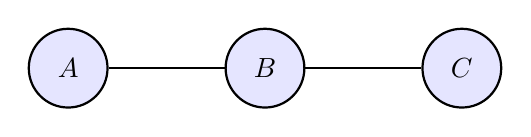
\begin{tikzpicture}[node distance=2.5cm, thick, scale=1.0, every node/.style={transform shape}]
    \node[circle, draw, fill=blue!10, minimum size=1cm] (A) {$A$};
    \node[circle, draw, fill=blue!10, minimum size=1cm, right of=A] (B) {$B$};
    \node[circle, draw, fill=blue!10, minimum size=1cm, right of=B] (C) {$C$};
    
    \draw (A) -- (B);
    \draw (B) -- (C);
\end{tikzpicture}
\caption{Undirected Graphical Model for $(A, B, C)$}
\label{fig:ugm_abc}
\end{figure}

\subsubsection*{\normalfont}{$\therefore$ The undirected graphical model , seen above, encodes the relationship that $A$ and $C$ are conditionally independent given $B$.}

\noindent\rule{\textwidth}{0.4pt}\\

\newpage

%------------------
% Solution for 3 (a)
%------------------
\subsection*{Solution 3}
\noindent\rule{\textwidth}{0.4pt}\\
\subsubsection*{Solution 3 (a)}
From the Hammersley-Clifford theorem, the joint probability distribution $P$ that factors over an undirected graph $G$ can be written as a product of potential functions ($\psi_C$) over the maximal cliques of the graph.
\begin{flushleft}
    Given, four random variables $W, X, Y, Z$ factor over the graph shown below.
\end{flushleft}
\begin{center}
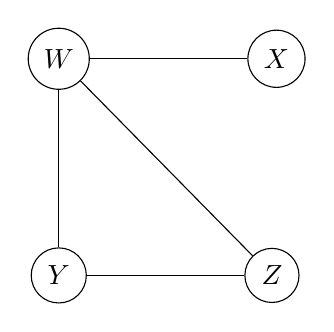
\begin{tikzpicture}[node distance=2cm]
\node[circle,draw] (W) {$W$};
\node[circle,draw,right=of W] (X) {$X$};
\node[circle,draw,below=of W] (Y) {$Y$};
\node[circle,draw,right=of Y] (Z) {$Z$};
\draw (W) -- (X);
\draw (Y) -- (W);
\draw (Y) -- (Z);
\draw (W) -- (Z);
\end{tikzpicture}
\end{center}
By inspection of the graph above the two maximal cliques are:
\begin{itemize}
    \item The triangle $\{W, Y, Z\}$
    \item The edge $\{W, X\}$
\end{itemize}
Hence, all other cliques, 
$$\{W, Y\}, \{W, Z\}, \text{ and } \{Y, Z\}$$
\begin{flushleft}
    are not maximal, as they are all subsets of the larger clique $\{W, Y, Z\}$.
\end{flushleft}


The joint distribution is the product of potentials over these two maximal cliques, normalized by the partition function $Z$.

\subsubsection*{\normalfont}{$\therefore$ The functional form is $P(W, X, Y, Z)$ ,where $Z$ is the partition function, is defined as:}
$$
P(W, X, Y, Z) = \frac{1}{Z} \psi_1(W, X) \psi_2(W, Y, Z) \text{ such that } Z = \sum_{w,x,y,z} \psi_1(w, x) \psi_2(w, y, z)
$$

\noindent\rule{\textwidth}{0.4pt}\\

\newpage

%------------------
% Solution for 3 (b)
%------------------
\subsection*{Solution 3}
\noindent\rule{\textwidth}{0.4pt}\\
\subsubsection*{Solution 3 (b)}
\begin{flushleft}
    Given, four random variables $W, X, Y, Z$ factor over the graph shown below.
\end{flushleft}
\begin{center}
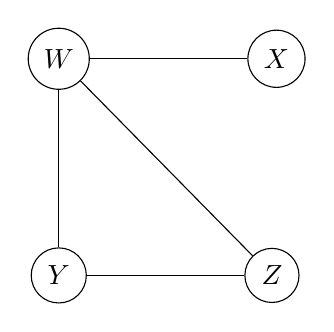
\begin{tikzpicture}[node distance=2cm]
\node[circle,draw] (W) {$W$};
\node[circle,draw,right=of W] (X) {$X$};
\node[circle,draw,below=of W] (Y) {$Y$};
\node[circle,draw,right=of Y] (Z) {$Z$};
\draw (W) -- (X);
\draw (Y) -- (W);
\draw (Y) -- (Z);
\draw (W) -- (Z);
\end{tikzpicture}
\end{center}
\begin{flushleft}
    Let, $A = \{X\}$ and $B = \{Y, Z\}$
\end{flushleft}
\begin{flushleft}
    Now, check all paths from $A$ to $B$ to see if $C = \{W\}$ is a separating set.
\end{flushleft}

\begin{enumerate}
    \item Paths from $X$ to $Y$ are 
    $$X\rightarrow W \rightarrow Y \text{ and } X \rightarrow W \rightarrow Z \rightarrow Y$$ 
    \item Paths from $X$ to $Z$ are: 
    $$X \rightarrow W \rightarrow Z \text{ and } X \rightarrow W \rightarrow Y \rightarrow Z$$ 
\end{enumerate}
\begin{flushleft}
    
\end{flushleft}
Hence, every possible path from $X$ must pass through the node $W$ to travel to any node in $\{Y, Z\}$. The set $C=\{W\}$ separates $A=\{X\}$ from $B=\{Y, Z\}$.

\subsubsection*{\normalfont}{$\therefore$ The distribution must satisfy the conditional independence property:}
$$X \perp \{Y, Z\} \mid W$$

\noindent\rule{\textwidth}{0.4pt}\\

\newpage

%------------------
% Solution for 4(a)
%------------------
\subsection*{Solution 4}
\noindent\rule{\textwidth}{0.4pt}\\
\subsubsection*{Solution 4 (a)}
\begin{flushleft}
    Given, the joint distribution $P$ over $(x_1, x_2, x_3)$ is given by the following table:
\end{flushleft}
\begin{center}
\begin{tabular}{c|c|c|c}
$x_1$ & $x_2$ & $x_3$ & Pr \\\hline
0 & 0 & 0 & 1/3 \\
0 & 0 & 1 & 1/3 \\
1 & 0 & 0 & 1/6 \\
1 & 1 & 1 & 1/6
\end{tabular}
\end{center}
\begin{flushleft}
    To check if variable $Y$ is a deterministic function of $X$ and $Z$, we check if, for every pair of values $(x, z)$ that has a non-zero probability of occurring, there is only one possible value for $y$.
\end{flushleft}

\begin{enumerate}
    \item Test $x_1 = f(x_2, x_3)$
    \begin{itemize}
        \item Row 1: $(x_2=0, x_3=0)$ maps to $x_1=0$.
        \item Row 3: $(x_2=0, x_3=0)$ maps to $x_1=1$.
    \end{itemize}
    Hence, this single input maps to two different outputs.

    \item Test $x_3 = f(x_1, x_2)$
    \begin{itemize}
        \item Row 1: $(x_1=0, x_2=0)$ maps to $x_3=0$.
        \item Row 2: $(x_1=0, x_2=0)$ maps to $x_3=1$.
    \end{itemize}
    Hence, this single input maps to two different outputs.

    \item $x_2 = f(x_1, x_3)$
    \begin{itemize}
        \item Row 1: Input $(x_1=0, x_3=0)$ maps to $x_2=0$.
        \item Row 2: Input $(x_1=0, x_3=1)$ maps to $x_2=0$.
        \item Row 3: Input $(x_1=1, x_3=0)$ maps to $x_2=0$.
        \item Row 4: Input $(x_1=1, x_3=1)$ maps to $x_2=1$.
    \end{itemize}
    In every case, a given input pair $(x_1, x_3)$ maps to a single, unique output for $x_2$.
\end{enumerate}

\subsubsection*{\normalfont}{$\therefore$ The deterministic relationship is:} 
$$x_2 = x_1 \land x_3 \quad (\text{i.e., }x_2 \text{ is } 1 \iff x_1=1 \text{ and } x_3=1)$$

\noindent\rule{\textwidth}{0.4pt}\\

\newpage

%------------------
% Solution for 4(b)
%------------------
\subsection*{Solution 4}
\noindent\rule{\textwidth}{0.4pt}\\
\subsubsection*{Solution 4 (b)}
From \textit{part (a)}, $x_2$ is a deterministic function of $x_1$ and $x_3$, defined as:
$$x_2 = x_1 \land x_3$$
\begin{flushleft}
    This means $P(x_2 \mid x_1, x_3)$ is deterministic. This strongly suggests a structure where $x_1$ and $x_3$ are parents of $x_2$.
\end{flushleft}
\begin{flushleft}
    This implies the factorization: 
\end{flushleft}
$$P(x_1, x_2, x_3) = P(x_1)P(x_3)P(x_2 \mid x_1, x_3)$$

To test this independence, we first compute the marginals from the table:
\begin{itemize}
    \item Marginal $P(x_1)$:
        \begin{itemize}
            \item $\Pr(x_1=0) = \Pr(0,0,0) + \Pr(0,0,1) = 1/3 + 1/3 = 2/3$
            \item $\Pr(x_1=1) = \Pr(1,0,0) + \Pr(1,1,1) = 1/6 + 1/6 = 1/3$
        \end{itemize}
    \item Marginal $P(x_3)$:
        \begin{itemize}
            \item $\Pr(x_3=0) = \Pr(0,0,0) + \Pr(1,0,0) = 1/3 + 1/6 = 3/6 = 1/2$
            \item $\Pr(x_3=1) = \Pr(0,0,1) + \Pr(1,1,1) = 1/3 + 1/6 = 3/6 = 1/2$
        \end{itemize}
    \item Joint $P(x_1, x_3)$: (Sum over $x_2$)
        \begin{itemize}
            \item $\Pr(x_1=0, x_3=0) = \Pr(0,0,0) = 1/3$
            \item $\Pr(x_1=0, x_3=1) = \Pr(0,0,1) = 1/3$
            \item $\Pr(x_1=1, x_3=0) = \Pr(1,0,0) = 1/6$
            \item $\Pr(x_1=1, x_3=1) = \Pr(1,1,1) = 1/6$
        \end{itemize}
\end{itemize}
Now, check for independence: $\Pr(x_1, x_3) = \Pr(x_1)\Pr(x_3)$
\begin{itemize}
    \item $\Pr(x_1=0)\Pr(x_3=0) = (2/3)(1/2) = 1/3$. This equals $\Pr(x_1=0, x_3=0)$.
    \item $\Pr(x_1=0)\Pr(x_3=1) = (2/3)(1/2) = 1/3$. This equals $\Pr(x_1=0, x_3=1)$.
    \item $\Pr(x_1=1)\Pr(x_3=0) = (1/3)(1/2) = 1/6$. This equals $\Pr(x_1=1, x_3=0)$.
    \item $\Pr(x_1=1)\Pr(x_3=1) = (1/3)(1/2) = 1/6$. This equals $\Pr(x_1=1, x_3=1)$.
\end{itemize}
It follows that, $P(x_1, x_3) = P(x_1)P(x_3)$ holds for all combinations, $x_1$ and $x_3$ are marginally independent.
Hence, the minimal Bayes net is therefore the one that encodes $x_1 \perp x_3$ and the dependency $x_2 = f(x_1, x_3)$. This is the v-structure $x_1 \to x_2 \leftarrow x_3$.

\begin{center}
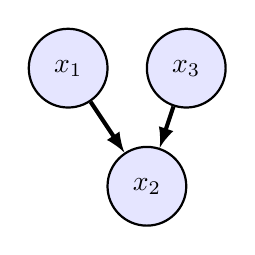
\begin{tikzpicture}[node distance=1.5cm and 2cm, thick]
    \node[circle, draw, fill=blue!10, minimum size=1cm] (x1) {$x_1$};
    \node[circle, draw, fill=blue!10, minimum size=1cm, right of=x1] (x3) {$x_3$};
    \node[circle, draw, fill=blue!10, minimum size=1cm, below of=x1, xshift=1cm] (x2) {$x_2$};
    
    \draw[->, >=latex, line width=1.5pt] (x1) -- (x2);
    \draw[->, >=latex, line width=1.5pt] (x3) -- (x2);
\end{tikzpicture}
\end{center}

\subsubsection*{\normalfont}{$\therefore$ The minimal Bayes net is the v-structure $x_1 \to x_2 \leftarrow x_3$, as $x_1$ and $x_3$ are marginally independent, and $x_2$ is a deterministic function of both.}

\noindent\rule{\textwidth}{0.4pt}\\

\newpage

%------------------
% Solution for 4(c)
%------------------
\subsection*{Solution 4}
\noindent\rule{\textwidth}{0.4pt}\\
\subsubsection*{Solution 4 (c)}
From \textit{part(b)}, we know the minimal Bayes net is the v-structure $x_1 \to x_2 \leftarrow x_3$. The joint distribution thus factors as:
$$ P(x_1, x_2, x_3) = P(x_1) P(x_3) P(x_2 \mid x_1, x_3) $$
This factorization yeilds three (Conditional) Probability Tables (CPTs).
\begin{enumerate}
    \item CPT for $x_1$: Find the marginal probability $P(x_1)$ by summing over $x_2$ and $x_3$ in the joint table.
    $$\Pr(x_1=0) = \Pr(0,0,0) + \Pr(0,0,1) = \frac{1}{3} + \frac{1}{3} = \frac{2}{3}$$
    $$\Pr(x_1=1) = \Pr(1,0,0) + \Pr(1,1,1) = \frac{1}{6} + \frac{1}{6} = \frac{1}{3}$$
    \begin{center}
    \begin{tabular}{c|c}
    $x_1$ & $\Pr(x_1)$ \\\hline
    0 & 2/3 \\
    1 & 1/3
    \end{tabular}
    \end{center}
    \item CPT for $x_3$: Find the marginal probability $P(x_3)$ by summing over $x_1$ and $x_2$.
    $$\Pr(x_3=0) = \Pr(0,0,0) + \Pr(1,0,0) = \frac{1}{3} + \frac{1}{6} = \frac{1}{2}$$
    $$\Pr(x_3=1) = \Pr(0,0,1) + \Pr(1,1,1) = \frac{1}{3} + \frac{1}{6} = \frac{1}{2}$$
    \begin{center}
    \begin{tabular}{c|c}
    $x_3$ & $\Pr(x_3)$ \\\hline
    0 & 1/2 \\
    1 & 1/2
    \end{tabular}
    \end{center}
    \item CPT for $x_2$:From \textit{part (a)}, $x_2 = x_1 \land x_3$. This conditional probability is deterministic.
    \begin{center}
    \begin{tabular}{cc|c|c}
    $x_1$ & $x_3$ & $\Pr(x_2=0 \mid x_1, x_3)$ & $\Pr(x_2=1 \mid x_1, x_3)$ \\\hline
    0 & 0 & 1 & 0 \\
    0 & 1 & 1 & 0 \\
    1 & 0 & 1 & 0 \\
    1 & 1 & 0 & 1
    \end{tabular}
    \end{center}

\end{enumerate}

\subsubsection*{\normalfont}{$\therefore$ The three tables are $P(x_1)$ (with $\Pr(x_1=1)=1/3$), $P(x_3)$ (with $\Pr(x_3=1)=1/2$), and the deterministic CPT for $P(x_2 \mid x_1, x_3)$ which implements the $x_2 = x_1 \land x_3$ function.}

\noindent\rule{\textwidth}{0.4pt}\\

\newpage

%------------------
% Solution for 4(d)
%------------------
\subsection*{Solution 4}
\noindent\rule{\textwidth}{0.4pt}\\
\subsubsection*{Solution 4 (d)}
To find the minimal undirected graph (UGM), we "moralize" the minimal Bayes net from \textit{part (b)}.

\begin{enumerate}
    \item Start with the Bayes Net: From \textit{part (b)}, the graph was the v-structure $x_1 \to x_2 \leftarrow x_3$.

    \item Add moral edge: The nodes $x_1$ and $x_3$ are both parents of $x_2$. We must add an undirected edge between them.

    \item Drop Arrowheads: Convert all directed edges ($x_1 \to x_2$ and $x_3 \to x_2$) into undirected edges.
\end{enumerate}
\begin{flushleft}
    This process results in a fully connected graph (a 3-clique) with edges $(x_1, x_2)$, $(x_2, x_3)$, and the new moral edge $(x_1, x_3)$.
\end{flushleft}

\begin{center}
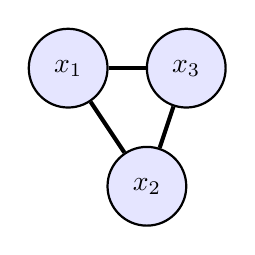
\begin{tikzpicture}[node distance=1.5cm and 2cm, thick]
    \node[circle, draw, fill=blue!10, minimum size=1cm] (x1) {$x_1$};
    \node[circle, draw, fill=blue!10, minimum size=1cm, right of=x1] (x3) {$x_3$};
    \node[circle, draw, fill=blue!10, minimum size=1cm, below of=x1, xshift=1cm] (x2) {$x_2$};
    
    \draw[line width=1.5pt] (x1) -- (x2);
    \draw[line width=1.5pt] (x3) -- (x2);
    \draw[line width=1.5pt] (x1) -- (x3);
\end{tikzpicture}
\end{center}

\subsubsection*{\normalfont}{$\therefore$ The minimal undirected graph can be seen above.}

\noindent\rule{\textwidth}{0.4pt}\\

\newpage

%------------------
% Solution for 5(a)
%------------------
\subsection*{Solution 5}
\noindent\rule{\textwidth}{0.4pt}\\
\subsubsection*{Solution 5 (a)}
The joint distribution from the notebook is:
$$
\Pr(X,Y) \propto \exp\left( \sum_p X_p Y_p + \sum_{p \sim q} Y_p Y_q \right)
$$
For Gibbs sampling, the full conditional probability $\Pr(Y_p \mid Y_{\backslash p}, X)$ is proportional to all terms in the joint distribution that involve $Y_p$:
\begin{align*}
    \Pr(Y_p \mid Y_{\backslash p}, X) &\propto \exp\left( X_p Y_p + \sum_{q \in \mathcal{N}(p)} Y_p Y_q \right)
\end{align*}
where $\mathcal{N}(p)$ is the set of neighbors of pixel $p$. We can factor out $Y_p$:
$$
\Pr(Y_p \mid Y_{\backslash p}, X) \propto \exp\left( Y_p \cdot \left( X_p + \sum_{q \in \mathcal{N}(p)} Y_q \right) \right)
$$
The local evidence is defined as:
$$E_p = X_p + \sum_{q \in \mathcal{N}(p)} Y_q$$
Substituting $E_p$ the equation simplifies to:
$$
\Pr(Y_p \mid Y_{\backslash p}, X) \propto \exp( Y_p E_p )
$$
Now, normalize over the two possible states $Y_p \in \{-1, +1\}$:

$$\Pr(Y_p = +1 \mid \ldots) = \frac{\exp( (+1) \cdot E_p )}{\exp( (+1) \cdot E_p ) + \exp( (-1) \cdot E_p )} = \frac{e^{E_p}}{e^{E_p} + e^{-E_p}}$$

Finally, multiply the numerator and denominator by $e^{-E_p}$ (1) and we arrive at the following:
$$
\Pr(Y_p = +1 \mid \ldots) = \frac{1}{1 + e^{-2E_p}}
$$

\subsubsection*{\normalfont}{$\therefore$ The precise expression is:}
$$\Pr(Y_p = +1 \mid Y_{\backslash p}, X) = \frac{1}{1 + \exp(-2 E_p)} \quad \text{,where } E_p = X_p + \sum_{q \in \mathcal{N}(p)} Y_q$$

\noindent\rule{\textwidth}{0.4pt}\\

\newpage

%------------------
% Solution for 5(b)
%------------------
\subsection*{Solution 5}
\noindent\rule{\textwidth}{0.4pt}\\
\subsubsection*{Solution 5 (b)}
\subsubsection*{Python Code: Gibbs sampler}
\begin{lstlisting}
import numpy as np
import matplotlib.pyplot as plt
import cv2
import math

def load_image(filename):
  img = cv2.imread(filename,cv2.IMREAD_GRAYSCALE)
  img = img/255.0
  img[img>=0.5]=1.0
  img[img<0.5]=0.0
  img = img*2-1
  return img

# Load in both the degraded image and the original
img = load_image("noisy_bear.png")
gt = load_image("original_bear.png")
M,N = img.shape[0], img.shape[1]

# Create a version of img that is padded with zeros all around
padded_image = np.zeros((img.shape[0]+2, img.shape[1]+2)) #Padding image to make some computations easier 
padded_image[1:-1,1:-1] = img

def gibbs_step(Y, X):
    Y_new = np.copy(Y)
    M, N = Y.shape
    
    # loop over every pixel
    for i in range(M):
        for j in range(N):
            # sum over neighbors
            neighbors_sum = 0
            if i > 0:   neighbors_sum += Y_new[i-1, j] 
            if i < M-1: neighbors_sum += Y_new[i+1, j] 
            if j > 0:   neighbors_sum += Y_new[i, j-1] 
            if j < N-1: neighbors_sum += Y_new[i, j+1] 
            
            # E_p = eta * X_p + beta * neighbors_sum (eta=1 and beta=1)
            E_p = X[i, j] + neighbors_sum
            
            # prob of Y_p = +1 -> prob_plus_one = 1.0 / (1.0 + np.exp(-2.0 * E_p))
            if E_p * 2 > 700: # Avoid overflow in exp
                prob_plus_one = 1.0
            elif E_p * 2 < -700:
                prob_plus_one = 0.0
            else:
                prob_plus_one = 1.0 / (1.0 + np.exp(-2.0 * E_p))

            # sample from Bernoulli(prob_plus_one)
            if np.random.rand() < prob_plus_one:
                Y_new[i, j] = 1
            else:
                Y_new[i, j] = -1
                
    return Y_new

# initalize Y and set X to the img
X = img
Y = np.random.choice([-1, 1], size=X.shape)
num_iterations = 50
images_to_show = []
iterations_to_save = [0, 1, 5, 10, 49]

for t in range(num_iterations):
    if t in iterations_to_save:
        images_to_show.append(np.copy(Y))
    Y = gibbs_step(Y, X)

# plot
fig, axes = plt.subplots(1, len(images_to_show), figsize=(20, 4))
for ax, img, t in zip(axes, images_to_show, iterations_to_save):
    ax.imshow(img, cmap='gray')
    ax.set_title(f'Iteration {t}')
    ax.axis('off')
plt.show()
\end{lstlisting}

\subsubsection*{Images}
\begin{figure}[h]
  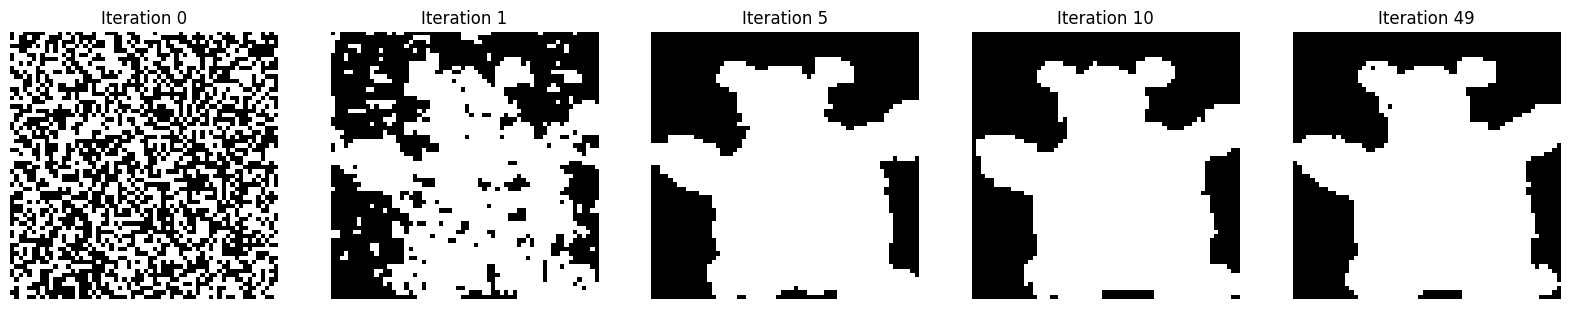
\includegraphics[width=\textwidth]{q5b.png}
  \caption{Image 0,1,5,10,49 while Markov chain is missing}
\end{figure}

\noindent\rule{\textwidth}{0.4pt}\\

\newpage

%------------------
% Solution for 5(c)
%------------------
\subsection*{Solution 5}
\noindent\rule{\textwidth}{0.4pt}\\
\subsubsection*{Solution 5 (c)}
\subsubsection*{Python Code: Reconstruct Image}
\begin{lstlisting}
import numpy as np
import matplotlib.pyplot as plt
def get_posterior_mean(Y, X, burn_in, num_samples):
    M, N = X.shape
    Y_samples_sum = np.zeros((M, N), dtype=float)
    
    # run the chain
    for t in range(burn_in + num_samples):
        Y = gibbs_step(Y, X)
        # After burn-in, start collecting samples
        if t >= burn_in:
            Y_samples_sum += Y        
    # calc average
    posterior_mean = Y_samples_sum / num_samples
    return posterior_mean

X= img
Y_init = np.random.choice([-1, 1], size=X.shape)
posterior_mean_image = get_posterior_mean(Y_init, X, burn_in=50, num_samples=200)

# plot
plt.imshow(posterior_mean_image, cmap='gray', vmin=-1, vmax=1)
plt.title('Reconstructed Image E[Y|X]')
plt.axis('off')
plt.show()
\end{lstlisting}

\subsubsection*{Reconstructed Image}
\begin{center}
  
\includegraphics[width=0.6\textwidth]{q5c.png} 
\end{center}

\noindent\rule{\textwidth}{0.4pt}\\

\newpage

%------------------
% Solution for 6(a)
%------------------
\subsection*{Solution 6}
\noindent\rule{\textwidth}{0.4pt}\\
\subsubsection*{Solution 6 (a)}
\subsubsection*{Python Code: Plot $f(x)$}
\begin{lstlisting}[language=Python]
import numpy as np
import matplotlib.pyplot as plt

# set the function and domain
f = lambda x: 0.5 * np.sin(x)
x_domain = np.linspace(0, np.pi, 400)
y_values = f(x_domain)

# plot
fig, ax = plt.subplots(figsize=(8, 5))
ax.plot(x_domain, y_values, 'r-', linewidth=2, 
        label=r'$f(x) = \frac{1}{2}\sin(x)$')
ax.set_xlabel('x (radians)', fontsize=12)
ax.set_ylabel('Density f(x)', fontsize=12)
ax.set_title('Target Probability Density Function', fontsize=14)
ax.legend(fontsize=10)
ax.grid(True, alpha=0.3)
ax.set_xlim(0, np.pi)
ax.set_ylim(0, 0.6) # Max is 0.5, give a little space
plt.savefig('q6a_plot.png', dpi=150, bbox_inches='tight')
plt.show()
\end{lstlisting}
\subsubsection*{Plot}
\begin{center}
  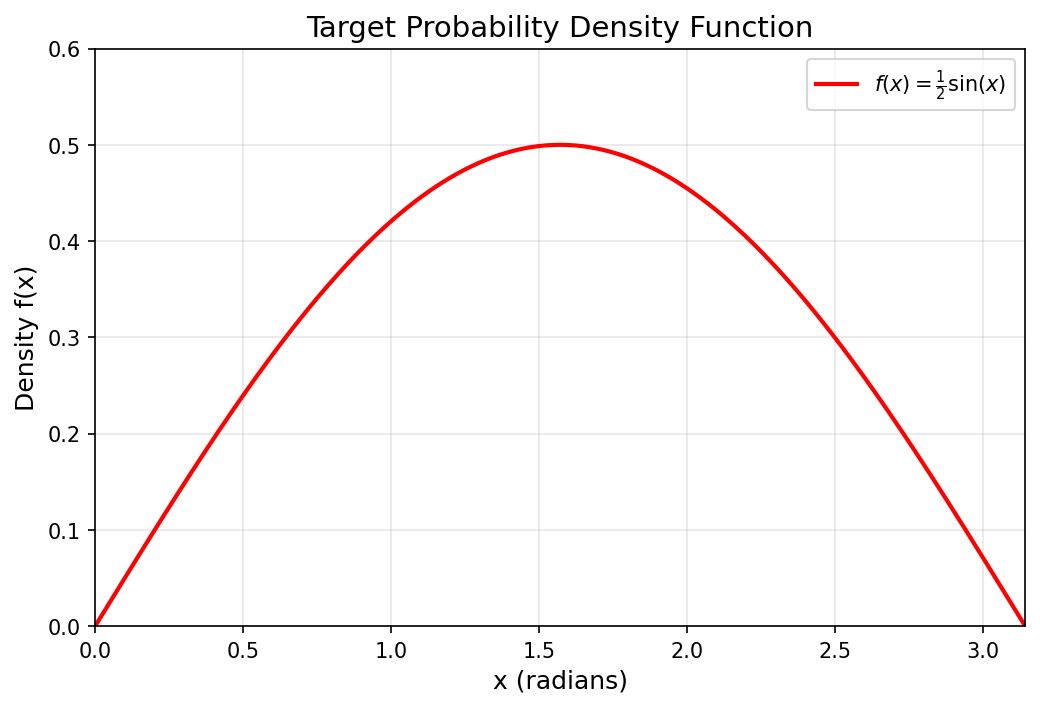
\includegraphics[width=0.6\textwidth]{q6a_plot.png} 
\end{center}

\noindent\rule{\textwidth}{0.4pt}\\
\newpage

%------------------
% Solution for 6(b)
%------------------
\subsection*{Solution 6}
\noindent\rule{\textwidth}{0.4pt}\\
\subsubsection*{Solution 6 (b)}
\begin{enumerate}
    \item Suitable Proposal $g(x)$
    The target density $f(x)$ is defined on the interval $[0, \pi]$. The simplest proposal distribution $g(x)$ that covers this support is the Uniform distribution on $[0, \pi]$.
    \begin{itemize}
        \item Its support, $[0, \pi]$, matches the support of $f(x)$.
        \item $f(x) > 0$ only when $x \in (0, \pi)$, and $g(x) > 0$ on this entire interval.
    \end{itemize}
The probability density function (PDF) for $g(x) = \text{Uniform}(0, \pi)$ is:
$$
g(x) = \frac{1}{\pi - 0} = \frac{1}{\pi} \quad \text{for } x \in [0, \pi]
$$
    \item Suitable Upper Bound $M$
We need to find the smallest constant $M$ such that $f(x) \le M g(x)$, which is equivalent to finding the maximum of the ratio $f(x)/g(x)$:
$$
M = \sup_{x \in [0, \pi]} \frac{f(x)}{g(x)}
$$
We compute this ratio:
$$
\frac{f(x)}{g(x)} = \frac{\frac{1}{2} \sin x}{\frac{1}{\pi}} = \frac{\pi}{2} \sin x
$$
To find the maximum, we find the maximum of $\sin x$ on the interval $[0, \pi]$, which is $1$ (at $x = \pi/2$).

Hence, the tightest possible upper bound $M$ is:
$$
M = \frac{\pi}{2} \cdot \left( \max_{x \in [0, \pi]} \sin x \right) = \frac{\pi}{2} \cdot 1 = \frac{\pi}{2}
$$
\end{enumerate}

\subsubsection*{\normalfont}{$\therefore$ A suitable proposal is $g(x) = \text{Uniform}(0, \pi)$ with PDF $g(x) = 1/\pi$. The corresponding tightest upper bound is $M = \frac{\pi}{2}$.}

\noindent\rule{\textwidth}{0.4pt}\\

\newpage

%------------------
% Solution for 6(c)
%------------------
\subsection*{Solution 6}
\noindent\rule{\textwidth}{0.4pt}\\
\subsubsection*{Solution 6 (c)}
\subsubsection*{Python Code: Rejection Sampler}
\begin{lstlisting}[language=Python]
import numpy as np

# set seed
np.random.seed(42)

N_ACCEPT = 10000
accepted_samples = []
total_draws = 0

# Parameters from part (b)
f = lambda x: 0.5 * np.sin(x)
g = lambda x: 1.0 / np.pi
M = np.pi / 2.0

# loop until we have 10,000 accepted samples
while len(accepted_samples) < N_ACCEPT:
    total_draws += 1
    
    # 1. Sample x from g(x) = Uniform(0, pi)
    x_proposal = np.random.uniform(0, np.pi)
    
    # 2. Sample u from Uniform(0, 1)
    u = np.random.rand()
    
    # 3. Calculate acceptance probability
    # p_accept = f(x) / (M * g(x)) = sin(x)
    acceptance_prob = np.sin(x_proposal)
    
    # 4. Accept/Reject
    if u <= acceptance_prob:
        accepted_samples.append(x_proposal)

# Print the results
print(f"Target number of samples: {N_ACCEPT}")
print(f"Total samples drawn from g: {total_draws}")
print(f"Empirical acceptance rate: {N_ACCEPT / total_draws:.4f}")
print(f"Theoretical acceptance rate (2/pi): {2.0 / np.pi:.4f}")

\end{lstlisting}

\subsubsection*{\normalfont}{$\therefore$ see output below}
\begin{verbatim}
Target number of samples: 10000
Total samples drawn from g: 15529
Empirical acceptance rate: 0.6440
Theoretical acceptance rate (2/pi): 0.6366
\end{verbatim}

\noindent\rule{\textwidth}{0.4pt}\\

\newpage

%------------------
% Solution for 6(d)
%------------------
\subsection*{Solution 6}
\noindent\rule{\textwidth}{0.4pt}\\
\subsubsection*{Solution 6 (d)}
We use the \texttt{accepted\_samples} list (containing 10,000 samples) that was generated in part 6(c). We use Matplotlib's \texttt{hist} function, specifying \texttt{bins=50} and, most importantly, \texttt{density=True}. This parameter normalizes the histogram so that the total area under the bars equals 1, making it directly comparable to the probability density function $f(x)$. We then overlay the plot of $f(x)$ from 6(a) to visually confirm the match.

\subsubsection*{Python Code: Plot Histogram}
\begin{lstlisting}[language=Python, caption={Python code to plot the histogram and true density.}]
import numpy as np
import matplotlib.pyplot as plt

# used samplesfrom part (c) 

# 1. Define the true function and domain (from 6a)
f = lambda x: 0.5 * np.sin(x)
x_domain = np.linspace(0, np.pi, 400)
y_true = f(x_domain)

# plot
fig, ax = plt.subplots(figsize=(8, 5))
ax.hist(accepted_samples, bins=50, density=True, 
        label='Sampled Histogram (10k samples)', 
        alpha=0.7, edgecolor='k', linewidth=0.5)
ax.plot(x_domain, y_true, 'r-', linewidth=3, 
        label=r'True Density $f(x) = \frac{1}{2}\sin(x)$')
ax.set_xlabel('x (radians)', fontsize=12)
ax.set_ylabel('Density', fontsize=12)
ax.set_title('Rejection Sampling: Histogram vs. True Density', fontsize=14)
ax.legend(fontsize=10)
ax.grid(True, alpha=0.3)
ax.set_xlim(0, np.pi)
plt.savefig('q6d_histogram.png', dpi=150, bbox_inches='tight')
plt.show()
\end{lstlisting}
\subsubsection*{Resulting Plot}
\begin{figure}[h!]
\centering
% This image is generated by the Python code above.
% Make sure to run the code to produce 'q6d_histogram.png'
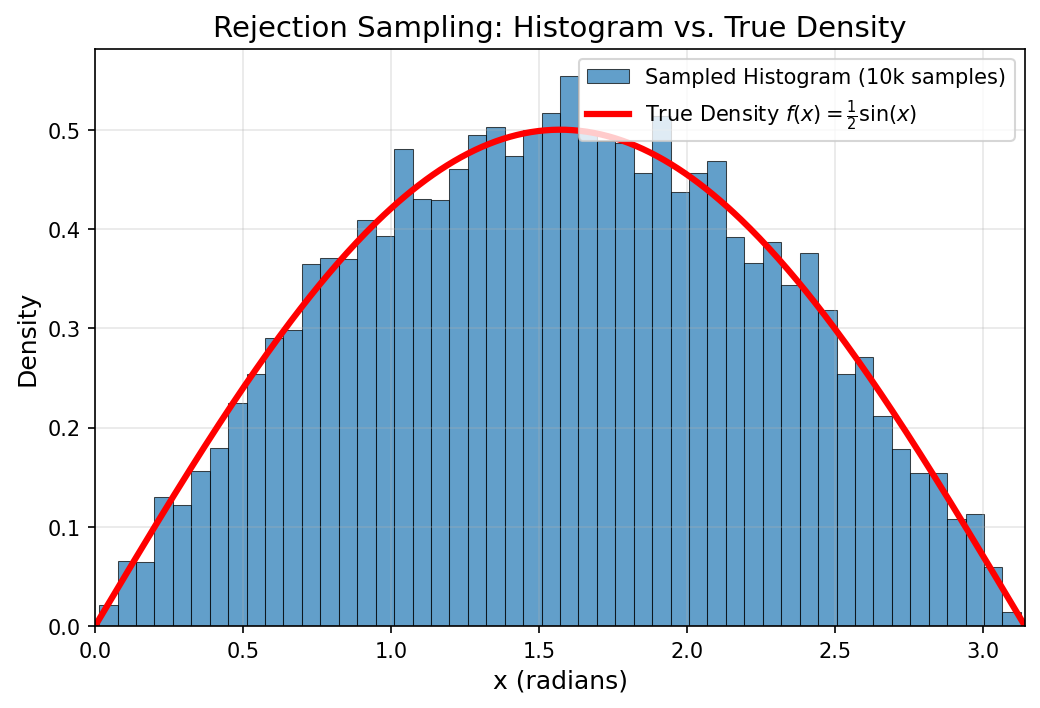
\includegraphics[width=0.7\textwidth]{q6d_histogram.png}
\caption{Normalized histogram of 10,000 accepted samples overlaid with the true target density $f(x)$.}
\label{fig:q6d_histogram}
\end{figure}

\end{document}
